\documentclass[
	% -- opções da classe memoir --
	12pt,				% tamanho da fonte
	%openright,			% capítulos começam em pág ímpar (insere página vazia caso preciso)
	oneside,			% para impressão em uma pagina por folha
	a4paper,			% tamanho do papel. 
	% -- opções do pacote babel --
	english,			% idioma adicional para hifenização
	french,				% idioma adicional para hifenização
	spanish,			% idioma adicional para hifenização
	brazil				% o último idioma é o principal do documento
	]{Dissertacao}
\usepackage{babel}[portuguese]
\usepackage[T1]{fontenc}		% Selecao de codigos de fonte.
\usepackage[utf8]{inputenc}		% Codificacao do documento (conversão automática dos acentos)
\usepackage{graphicx}

%\usepackage{lastpage}			% Usado pela Ficha catalográfica
\usepackage{indentfirst}		% Indenta o primeiro parágrafo de cada seção.
\usepackage{multirow}
\usepackage[table,xcdraw]{xcolor}
\usepackage{color}				% Controle das cores
\usepackage{graphicx}			% Inclusão de gráficos
\usepackage{microtype} 			% para melhorias de justificação
\usepackage{acronym}            %inclusao de acronimos

\definecolor{mygreen}{rgb}{0,0.6,0}
\definecolor{mygray}{rgb}{0.5,0.5,0.5}
\definecolor{mymauve}{rgb}{0.58,0,0.82}

\usepackage{listings}
\lstset{
   basicstyle=\ttfamily,
}


%modelo 
% para adaptações de elementos pré-textuais para UFMA
% ---
\usepackage{amsmath}            %para calculos
% ---
% Pacotes adicionais, usados apenas no âmbito do Modelo Canônico do abnteX2
% ---
\usepackage{lipsum}				% para geração de dummy text
% ---

% ---
% Pacotes de citações
% ---
%\usepackage[brazilian,hyperpageref]{backref}	 % Paginas com as citações na bibl
\usepackage[pagebackref]{hyperref}
\usepackage[hyphenbreaks]{breakurl}
\usepackage[alf,abnt-etal-list=0,abnt-etal-cite=2,abnt-emphasize=bf]{abntex2cite}
%\usepackage[sort&compress]{natbib}      % for bibliography
\setlength\bibindent{2em}


% Citações padrão ABNT

% --- 
% CONFIGURAÇÕES DE PACOTES
% --- 

% ---
% Configurações do pacote backref
% Usado sem a opção hyperpageref de backref
\renewcommand{\backrefpagesname}{Citado na(s) página(s):~}
% Texto padrão antes do número das páginas
\renewcommand{\backref}{}
% Define os textos da citação
\renewcommand*{\backrefalt}[4]{
	\ifcase #1 %
		Nenhuma citação no texto.%
	\or
		Citado na página #2.%
	\else
		Citado #1 vezes nas páginas #2.%
	\fi}%
% ---

% alterando o aspecto da cor azul
\definecolor{blue}{RGB}{41,5,195}
% --- 

% Espaçamentos entre linhas e parágrafos 
% O tamanho do parágrafo é dado por:
\setlength{\parindent}{1.3cm}

% Controle do espaçamento entre um parágrafo e outro:
\setlength{\parskip}{0.2cm}  % tente também \onelineskip

% ---
% compila o indice
% ---
\makeindex
% ---

% ----
% Início do documento
% ----
\begin{document}

% Retira espaço extra obsoleto entre as frases.
\frenchspacing 

% ----------------------------------------------------------
% ELEMENTOS PRÉ-TEXTUAIS
% ----------------------------------------------------------
% \pretextual

%%%%%%%%%%%%%%%%%%%%%%%%%%%%%%%%%%%
%							
% 	CAPA - FOLHA DE ROSTO - FOLHA DE APROVAÇÃO			  	  				
%
%%%%%%%%%%%%%%%%%%%%%%%%%%%%%%%%%%%

%----------------- Título e dados do autor
\titulo{Título do trabalho}
\autor{JOHN WICK}
\nome{John}
\ultimonome{Wick}

%----------------- Informações sobre curso e data
\mestrado

\curso{Ciência da Computação}
\ano{2020}
\data{10 de Abril de 2020} 
\cidade{São Luís}

%----------------- Informações sobre a instituição
\instituicao{Universidade Federal do Maranhão}
\sigla{UFMA}
\unidadeacademica{Centro de Ciências Exatas e Tecnologia}
\CDU{XXX.XXX \newline}

\areas{1.palavra-chave 2.palavra-chave 3.palavra-chave 4.palavra-chave 5.palavra-chave}
\npaginas{100}


%----------------- Informações banca examinadora
\orientador{John Wick (Orientador)}
\ttorientador{Doutor em Informática - UFMA}

\examinadorum{Membro Interno}
\ttexaminadorum{Doutor em Ciência da Computação - UFMA} 

\examinadordois{Membro Externo}
\ttexaminadordois{Doutor em Ciências da Computação - UFRJ} 

%\examinadortres{Prof. 3, Dr.} % Pode ser orientador por exemplo
%\ttexaminadortres{(Membro da Banca Examinadora)} 

%-----------------
\maketitle

% ----------------------------------------------------------
% Dedicatória
% ----------------------------------------------------------
% ---
\begin{dedicatoria}
   \vspace*{\fill}
   %\centering
   \noindent
   \begin{flushright}
   \textit{"Dedico a todos..."} 
   \end{flushright}
   %\vspace*{\fill}
\end{dedicatoria}
% ---

% ----------------------------------------------------------
% Agradecimentos
% ----------------------------------------------------------
% ---
\agradecimento{Agradecimentos}
A todos, os meus sinceros agradecimentos.

% ---

% ----------------------------------------------------------
% Epígrafe
% ----------------------------------------------------------
% ---
\begin{epigrafe}
    \vspace*{\fill}
	\begin{flushright}
		\textit{``“You Wanted Me Back...\\I’m Back!”.'' \\
		(John Wick)}
	\end{flushright}
\end{epigrafe}
% ---

% ----------------------------------------------------------
% RESUMOS
% ----------------------------------------------------------
% Em Português
\resumo{Resumo}

O problema abordado neste trabalho.

 \noindent \textbf{Palavras-chave}: palavra chave 1;palavra chave 2;palavra chave 3;palavra chave 4;palavra chave 4;palavra chave 5;palavra chave 6

% Em inglês
\resumo{Abstract}
 
The problem addressed in this work is...
 
\noindent \textbf{Key-words}: key word1; key word2; key word3;key word4; key word5; key word6

% inserir lista de acronimos
\cleardoublepage
\begingroup
\makeatletter
\let\ps@plain\ps@empty
\makeatother

\pagestyle{empty}
\addcontentsline{toc}{chapter}{Lista de Siglas}

\chapter*{Lista de Siglas}

\begin{acronym}

\acro{AI}{\emph{Articifial Intelligence} - Inteligência Artificial}
\acro{Cert.br}{Centro de Estudos, Resposta e Tratamento de Incidentes de Segurança no Brasil}
\acro{CNJ}{Conselho Nacional de Justiça}


\end{acronym}
\endgroup




% inserir lista de ilustrações
\emptypage
\listoffigures


% inserir lista de tabelas
%Lista de tabelas (Não-obrigatório)
\emptypage
\listoftables


% ----------------------------------------------------------
% Sumario
% ----------------------------------------------------------
%Sumário
\emptypage
\tableofcontents


% ----------------------------------------------------------
% ELEMENTOS TEXTUAIS
% ----------------------------------------------------------
%\textual

\pagestyle{ruledheader}


% ----------------------------------------------------------
% Capitulo 01
% ----------------------------------------------------------
%Introdução (exemplo de capítulo sem numeração, mas presente no Sumário)

% ----------------------------------------------------------
\chapter[Introdução]{Introdução}
% ----------------------------------------------------------

Aqui introdução do trabalho...

Exemplo de citação indireta: As informações concluiram isso \cite{schwab2016fourth}. 

Exemplo de utilização de acrônimos: Sistemas de \ac{AI}. Acrônimo detalha apenas na primeira utilização. Sistemas de \ac{AI}.

Palavra em itálico : \textit{backdoor}

Palavra em negrito : \textbf{backdoor}

Exmplo de citação direta: Segundo \citeonline{schwab2016fourth} o trabalho define..

\section{Objetivos}
Objetivo geral..

\subsection{Objetivos específicos}
Objetivos específicos..


\section{Organização do Trabalho}

No capítulo 2 ... No capítulo 3...

% ----------------------------------------------------------
% Capitulo 02
% ----------------------------------------------------------
\chapter[Fundamentação Teórica]{Fundamentação Teórica}

\begin{figure}[h]
\centering
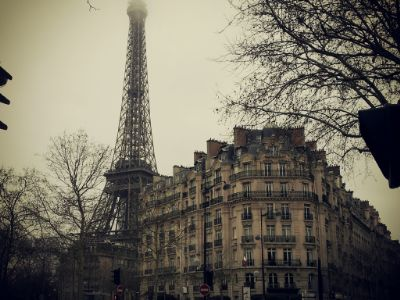
\includegraphics[width=.8\textwidth]{images/figura.jpg}
\caption{Exemplo de Imagem}
\label{fig:figura_1}
\end{figure}

Na Figura \ref{fig:figura_1}...

% ----------------------------------------------------------
% Capitulo 03
% ----------------------------------------------------------
\chapter[Trabalhos Relacionados]{Trabalhos Relacionados}



% ----------------------------------------------------------
% Capitulo 04
% ----------------------------------------------------------
\chapter[Proposta]{Proposta}



% ----------------------------------------------------------
% Capitulo 05
% ----------------------------------------------------------
\chapter[Experimentos]{Experimentos}



% ---
% Conclusão (outro exemplo de capítulo sem numeração e presente no sumário)
% ---
%Conclusão

\chapter{Conclusão, Publicações e Trabalhos Futuros}
%\addcontentsline{toc}{chapter}{Conclusão, Publicações e Trabalhos Futuros}
% ---

Este trabalho apresentou...

\section{Publicações}

Para divulgar os resultados obtidos..:
\begin{itemize}
    \item publicação....
    \textbf{Qualis Capes:} A2 pelo Qualis Capes.\\
    \textbf{Situação:} Publicado
\end{itemize}

\section{Trabalhos Futuros}

Como indicação de trabalhos futuros, sugerem-se :

\begin{enumerate}
    \item sugestão 1;
    
    \item sugestão 2;
    
    \item sugestão 3;
    
    \item sugestão 4;
    
    \item sugestão 5;
\end{enumerate}


% ----------------------------------------------------------
% ELEMENTOS PÓS-TEXTUAIS
% ----------------------------------------------------------
%\postextual
% ----------------------------------------------------------

% ----------------------------------------------------------
% Referências bibliográficas
% ----------------------------------------------------------

\bibliography{referencias}

\appendix
\chapter{Apêndice}
\section{Detalhes apêndice}

% ----------------------------------------------------------
% Glossário
% ----------------------------------------------------------
%
% Consulte o manual da classe abntex2 para orientações sobre o glossário.
%
%\glossary

%---------------------------------------------------------------------
% INDICE REMISSIVO
%---------------------------------------------------------------------
%\phantompart
%\printindex
%---------------------------------------------------------------------

\end{document}
